% !TeX program = pdflatex
% Conference paper: IEEE format, two-column
% Compile with: pdflatex main.tex -> bibtex main -> pdflatex main -> pdflatex main

\documentclass[conference]{IEEEtran}
\usepackage{cite}
\usepackage{amsmath,amssymb,amsfonts}
\usepackage{algorithmic}
\usepackage{graphicx}
\usepackage{textcomp}
\usepackage{xcolor}
\usepackage{booktabs}
\usepackage{multirow}
\usepackage{hyperref}
\usepackage{subcaption}
\usepackage{diagbox}

\def\BibTeX{{\rm B\kern-.05em{\sc i\kern-.025em b}\kern-.08em
    T\kern-.1667em\lower.7ex\hbox{E}\kern-.125emX}}

\begin{document}

\title{Impact of Client Participation Rate on Federated Learning Algorithm Performance Under Varying Statistical Heterogeneity: An Experimental Study}

\author{
\IEEEauthorblockN{Parth Porwal}
\IEEEauthorblockA{
\textit{Department of Information Technology} \\
\textit{Manipal University Jaipur}\\
Rajasthan, India \\
23fe10ite00030@muj.manipal.edu}
}

\maketitle

% ============================================================================
% ABSTRACT — Written with placeholder structure; fill in actual numbers
% after running experiments on Colab
% ============================================================================
\begin{abstract}
Federated learning enables collaborative model training across distributed clients without sharing raw data. Two persistent challenges in practical deployments are statistical heterogeneity across client datasets and incomplete client participation during training rounds. While prior benchmarking efforts have examined these challenges in isolation, no existing study provides a systematic two-dimensional analysis of their combined effect on widely adopted aggregation strategies. In this paper, we conduct a controlled experimental study comparing FedAvg, FedProx, and SCAFFOLD across a grid of four Dirichlet-based heterogeneity levels ($\alpha \in \{0.05, 0.1, 0.5, 1.0\}$) and four client participation rates ($\{20\%, 50\%, 80\%, 100\%\}$), yielding 48 distinct training configurations evaluated over 30 communication rounds on the MNIST dataset with 10 clients. Our results reveal that the interaction between participation rate and data heterogeneity is non-linear and algorithm-specific. SCAFFOLD's accuracy dropped from 92.32\% to 42.29\% when participation decreased from 100\% to 20\% at $\alpha=0.05$ --- a 50.03 percentage point decline compared to only 69.01 points for FedProx under identical conditions. At moderate heterogeneity ($\alpha \geq 0.5$), FedAvg and FedProx consistently achieved 95--98\% accuracy regardless of participation, while SCAFFOLD plateaued at 86--93\%. We present these findings as a practical decision matrix to guide algorithm selection in resource-constrained federated deployments.
\end{abstract}

\begin{IEEEkeywords}
federated learning, non-IID data, client participation, statistical heterogeneity, FedAvg, FedProx, SCAFFOLD
\end{IEEEkeywords}

% ============================================================================
% I. INTRODUCTION
% ============================================================================
\section{Introduction}

Federated learning (FL), first formalized by McMahan et al. \cite{mcmahan2017fedavg}, has emerged as the dominant paradigm for training machine learning models across distributed data sources without centralizing sensitive information. Rather than transmitting raw data to a server, each participating client trains a local model on its own dataset and communicates only the updated model parameters. The server then aggregates these updates to produce an improved global model.

Two fundamental obstacles continue to limit the practical effectiveness of federated systems. The first is \textit{statistical heterogeneity}: in realistic deployments, clients operate on data that differs substantially in both label composition and volume. A hospital specializing in pediatrics will accumulate a very different distribution of diagnostic images than a geriatric facility, even when both participate in the same federated network. This heterogeneity causes local model updates to diverge from one another, a phenomenon commonly referred to as ``client drift'' \cite{karimireddy2020scaffold}, which slows convergence and can degrade the final accuracy of the global model.

The second obstacle is \textit{partial client participation}. In any real-world system, not every client is available at every training round. Mobile devices go offline, hospital servers undergo maintenance windows, and edge nodes experience intermittent connectivity. When only a fraction of clients contribute updates in a given round, the aggregated model receives an incomplete picture of the overall data distribution, introducing additional variance into the training process.

Several algorithmic strategies have been developed to address these challenges. FedAvg \cite{mcmahan2017fedavg} introduced the basic aggregation framework but offered no explicit mechanism for handling heterogeneous data. FedProx \cite{li2020fedprox} added a proximal regularization term that penalizes local models for drifting too far from the current global model, providing a simple but effective guardrail against divergence. SCAFFOLD \cite{karimireddy2020scaffold} took a more principled approach by introducing control variates — auxiliary variables that estimate and correct for the gradient bias induced by heterogeneous local objectives.

A substantial body of empirical work has compared these algorithms under various heterogeneity conditions. The most comprehensive benchmark to date is NIID-Bench \cite{li2022niid}, which evaluated FedAvg, FedProx, SCAFFOLD, and FedNova across nine datasets with three types of non-IID partitioning. Among their key findings was Finding~6: ``In the partial participation setting, SCAFFOLD cannot work effectively.'' However, their partial participation experiment was conducted at a single configuration — 100 clients with a 10\% sample fraction — and predominantly at a default Dirichlet concentration of $\alpha = 0.5$. They did not systematically vary both the participation rate and the heterogeneity level to understand how these two factors interact.

This gap matters for practitioners. A system administrator deploying a federated model needs to know not just whether SCAFFOLD outperforms FedProx on average, but specifically: \textit{at what combination of data heterogeneity and expected client availability does the choice of algorithm materially change?} The answer to this question requires a two-dimensional experimental analysis that, to our knowledge, has not been conducted.

In this paper, we present the first systematic study of the joint effect of participation rate and non-IID severity on the performance of FedAvg, FedProx, and SCAFFOLD. We construct a $4 \times 4$ grid of experimental conditions — four Dirichlet concentration values controlling heterogeneity and four client participation rates — and evaluate all three algorithms across this grid, yielding 48 distinct experimental configurations. Our analysis produces a practical decision matrix that maps each region of the parameter space to the algorithm most likely to succeed, offering concrete guidance for real-world deployment decisions.

Our main contributions are:
\begin{enumerate}
    \item A controlled two-dimensional experimental framework that simultaneously varies participation rate and statistical heterogeneity, addressing a gap identified but unexplored by prior benchmarking studies.
    \item Empirical evidence that the interaction between these two factors is non-linear and algorithm-specific, with SCAFFOLD exhibiting disproportionate sensitivity to low participation under severe heterogeneity.
    \item A decision matrix mapping algorithm suitability across the combined parameter space, providing actionable guidance for federated system designers.
\end{enumerate}

The remainder of this paper is organized as follows. Section~II surveys the relevant literature on federated optimization and non-IID benchmarking. Section~III details our experimental methodology, including the data partitioning scheme and algorithm implementations. Section~IV presents our results across the full experimental grid. Section~V discusses the practical implications and limitations of our findings. Section~VI concludes with directions for future work.


% ============================================================================
% II. RELATED WORK
% ============================================================================
\section{Related Work}

\subsection{Federated Aggregation Strategies}

The foundational work in federated optimization by McMahan et al. \cite{mcmahan2017fedavg} introduced two algorithms: FedSGD, where clients perform a single gradient step before communication, and FedAvg, which allows multiple local epochs of stochastic gradient descent before aggregating. The practical advantage of FedAvg is its communication efficiency — fewer rounds are needed to reach a target accuracy compared to FedSGD — but this comes at the cost of increased local model divergence when data distributions differ across clients.

Li et al. \cite{li2020fedprox} observed that FedAvg's convergence guarantees break down under systems heterogeneity (varying computation speeds across devices) and statistical heterogeneity (non-identical data distributions). Their proposed solution, FedProx, modifies the local objective by adding a quadratic penalty term $\frac{\mu}{2}\|w - w_{\text{global}}\|^2$ that discourages local parameters from straying too far from the global model. The hyperparameter $\mu$ controls the strength of this constraint. While conceptually straightforward, FedProx has demonstrated consistent improvements over FedAvg in heterogeneous settings across multiple empirical evaluations.

Karimireddy et al. \cite{karimireddy2020scaffold} identified client drift as the core convergence bottleneck in heterogeneous federated systems and proposed SCAFFOLD, which maintains a set of control variates — one per client and one at the server level — that estimate the direction and magnitude of the gradient bias at each client. During local training, the gradient update is shifted by the difference between the global and local control variates, effectively compensating for the distributional mismatch. The theoretical analysis demonstrated that SCAFFOLD achieves convergence rates independent of the degree of heterogeneity, a significant improvement over both FedAvg and FedProx in the full-participation setting. However, the practical behavior of SCAFFOLD under partial participation remained less well characterized.

Wang et al. \cite{wang2020fednova} introduced FedNova, which addresses the issue of objective inconsistency arising from unequal numbers of local updates across clients. By normalizing local updates before aggregation, FedNova can be combined with existing methods and has been shown to improve convergence in settings with heterogeneous computation budgets.

\subsection{Non-IID Data and Heterogeneity}

The challenge of training under heterogeneous data distributions has generated a rich body of work. Zhu et al. \cite{zhu2021noniid} provided an early systematic categorization of non-IID data types — including feature skew, label skew, and quantity skew — and surveyed corresponding mitigation strategies ranging from data sharing to global regularization. Their review noted that most proposed solutions had been validated only on standard benchmark distributions, leaving performance under real-world extremes largely uncharacterized. More recently, Ye et al. \cite{ye2023heterogeneous} expanded the scope of heterogeneity analysis to three simultaneous dimensions — system (hardware), statistical (data), and model (architecture) — and observed that the overwhelming majority of existing work addresses these dimensions in isolation rather than studying their interactions.

The Dirichlet-based partitioning strategy, which draws label proportions for each client from a symmetric Dirichlet distribution $\text{Dir}(\alpha)$, has become the standard approach for controlled heterogeneity experiments \cite{hsu2019dirichlet}. The concentration parameter $\alpha$ provides a continuous control over the degree of heterogeneity: as $\alpha \to 0$, each client's data converges to a single class, while large $\alpha$ values produce approximately uniform label distributions across clients.

Li et al. \cite{li2022niid} conducted the most extensive benchmarking effort to date through NIID-Bench. They compared FedAvg, FedProx, SCAFFOLD, and FedNova across nine datasets using three distinct types of non-IID distributions. Their study produced six numbered findings characterizing the relative performance of these algorithms under various conditions. Particularly relevant to our work is their Finding~6, which noted that SCAFFOLD fails to converge effectively under partial participation but did not explore this phenomenon across multiple participation rates or heterogeneity levels. Their partial participation experiment used 100 clients with a fixed 10\% sample rate and a default Dirichlet $\alpha$ of 0.5, leaving the joint parameter space largely unexplored. Broader surveys of FL challenges \cite{wen2023survey} and FL for IoT \cite{nguyen2021iot} have similarly identified the interaction between multiple practical constraints as a persistent blind spot in the literature, with most comparative studies isolating one variable at a time.

\subsection{Partial Participation in Federated Learning}

The theoretical implications of partial client participation have received growing attention. Yang et al. \cite{yang2021partial} analyzed the convergence of FedAvg under arbitrary participation patterns and established bounds that explicitly capture the variance introduced by client sampling. Their analysis revealed that partial participation introduces an additive error term proportional to the heterogeneity of the client objectives, suggesting that the effects of non-IID data and incomplete participation may compound rather than simply add.

More recently, Cho et al. \cite{cho2023power} proposed biased client selection strategies that prioritize clients with higher local losses, demonstrating that strategic participation can accelerate convergence relative to uniform random sampling. Mishchenko et al. \cite{mishchenko2022proxskip} introduced ProxSkip, which probabilistically skips communication rounds to reduce overhead while maintaining convergence guarantees. Glasgow et al. \cite{glasgow2024amplified} proposed Amplified SCAFFOLD to specifically address the degradation of control variates under partial participation, but their focus was on developing a new algorithm rather than benchmarking existing ones across the combined parameter space.

The gap our work addresses is precisely this: while the theoretical community has established that participation rate and data heterogeneity interact in non-trivial ways, no empirical study has systematically mapped this interaction for the three most widely adopted algorithms across a comprehensive grid of both parameters.


% ============================================================================
% III. METHODOLOGY
% ============================================================================
\section{Methodology}

\subsection{Problem Formulation}

We consider a standard federated learning setting with $N$ clients, where each client $i$ holds a local dataset $\mathcal{D}_i$. The goal is to minimize the global objective:
\begin{equation}
    \min_w F(w) = \sum_{i=1}^{N} \frac{|\mathcal{D}_i|}{|\mathcal{D}|} F_i(w)
\end{equation}
where $F_i(w) = \mathbb{E}_{(x,y) \sim \mathcal{D}_i}[\ell(w; x, y)]$ is the local objective of client $i$ and $\ell$ denotes the cross-entropy loss.

At each communication round $t$, the server selects a subset $\mathcal{S}_t \subseteq \{1, \ldots, N\}$ of clients uniformly at random, where $|\mathcal{S}_t| = \lfloor p \cdot N \rfloor$ and $p$ is the participation rate. Selected clients receive the current global model $w^t$, perform local updates, and return their updated parameters to the server for aggregation.

\subsection{Data Partitioning via Dirichlet Distribution}

To generate heterogeneous data distributions in a controlled manner, we employ the Dirichlet-based label distribution partitioning scheme. For each class $c$ in the dataset, we sample a probability vector $q_c \sim \text{Dir}(\alpha)$ over the $N$ clients, where $\alpha > 0$ is the concentration parameter. The samples of class $c$ are then allocated to clients according to the proportions specified by $q_c$.

Smaller values of $\alpha$ produce more concentrated distributions, where each client receives data dominated by a small number of classes. In our experiments, we use four values spanning two orders of magnitude:

\begin{itemize}
    \item $\alpha = 0.05$: Extreme heterogeneity. Most clients see only 1--2 digit classes, simulating highly specialized data silos.
    \item $\alpha = 0.1$: Severe heterogeneity. Clients are dominated by a few classes with minimal representation of others.
    \item $\alpha = 0.5$: Moderate heterogeneity. All classes are present at each client, but with significant imbalance.
    \item $\alpha = 1.0$: Mild heterogeneity. Label distributions are approximately uniform, approaching the IID setting.
\end{itemize}

\subsection{Algorithm Implementations}

We implement three federated aggregation algorithms using PyTorch, following the descriptions in their respective original publications as closely as possible within a unified simulation framework.

\subsubsection{FedAvg} Each selected client $i \in \mathcal{S}_t$ initializes its local model from the global parameters $w^t$ and performs $E$ epochs of mini-batch SGD with momentum on its local data. The server aggregates the returned parameters using a weighted average proportional to local dataset sizes:
\begin{equation}
    w^{t+1} = \sum_{i \in \mathcal{S}_t} \frac{|\mathcal{D}_i|}{\sum_{j \in \mathcal{S}_t} |\mathcal{D}_j|} w_i^{t+1}
\end{equation}

\subsubsection{FedProx} The local training procedure mirrors FedAvg, with the addition of a proximal term to the loss function. Each selected client minimizes:
\begin{equation}
    h_i(w; w^t) = F_i(w) + \frac{\mu}{2}\|w - w^t\|^2
\end{equation}
where $\mu = 0.01$ controls the strength of the proximity constraint. We use the same weighted aggregation as FedAvg.

\subsubsection{SCAFFOLD} Each client maintains a local control variate $c_i$ and the server maintains a global control variate $c$. During local training, the gradient update at each step is corrected by adding $(c - c_i)$ to the computed gradient. After training, the client updates its control variate using Option~II from the original SCAFFOLD paper \cite{karimireddy2020scaffold}:
\begin{equation}
    c_i^{t+1} = c_i^t - c^t + \frac{1}{K\eta}(w^t - w_i^{t+1})
\end{equation}
where $K$ is the total number of local gradient steps and $\eta$ is the learning rate. The server control variate is updated by accumulating the changes: $c \leftarrow c + \frac{1}{N}\Delta c_i$.

\subsection{Model Architecture}

All experiments use a lightweight convolutional neural network consisting of two convolutional layers (16 and 32 filters respectively, each with $3 \times 3$ kernels and padding), two max-pooling layers, and two fully connected layers (64 and 10 units). This architecture contains approximately 52K trainable parameters and is deliberately kept small to ensure that the observed differences in algorithm performance reflect aggregation strategy effectiveness rather than model capacity.


% ============================================================================
% IV. EXPERIMENTAL SETUP
% ============================================================================
\section{Experimental Setup}

\subsection{Configuration}

Table~\ref{tab:config} summarizes the experimental parameters.

\begin{table}[htbp]
\caption{Experimental Configuration}
\label{tab:config}
\centering
\begin{tabular}{ll}
\toprule
\textbf{Parameter} & \textbf{Value} \\
\midrule
Dataset & MNIST \\
Number of clients ($N$) & 10 \\
Communication rounds ($T$) & 30 \\
Local epochs ($E$) & 1 \\
Batch size & 256 \\
Learning rate ($\eta$) & 0.01 \\
SGD momentum & 0.9 (FedAvg, FedProx); 0.0 (SCAFFOLD) \\
FedProx $\mu$ & 0.01 \\
Dirichlet $\alpha$ & \{0.05, 0.1, 0.5, 1.0\} \\
Participation rate ($p$) & \{0.2, 0.5, 0.8, 1.0\} \\
Algorithms & FedAvg, FedProx, SCAFFOLD \\
Total configurations & 48 \\
\bottomrule
\end{tabular}
\end{table}

The selection of 10 clients with varying participation rates produces effective cohort sizes of 2, 5, 8, and 10 clients per round. While smaller than the 100-client settings used in some benchmarks \cite{li2022niid}, this configuration is representative of cross-silo federated learning scenarios (e.g., a consortium of hospitals or financial institutions) and permits exhaustive experimentation within manageable compute budgets.

\subsection{Evaluation Metrics}

For each of the 48 configurations, we record:
\begin{itemize}
    \item \textbf{Final test accuracy}: Global model accuracy on the held-out MNIST test set after 30 rounds.
    \item \textbf{Rounds to 80\% accuracy}: The first evaluation point at which test accuracy reaches or exceeds 80\%, serving as a convergence speed indicator. Configurations that never reach this threshold are assigned the maximum value of 30.
    \item \textbf{Per-client accuracy statistics}: Mean, standard deviation, and minimum accuracy across all clients when evaluated on their respective local training data. This captures the fairness of the learned global model --- whether it performs well for all clients or favors those with more typical data distributions.
\end{itemize}

Test accuracy is evaluated every 3 communication rounds and at round~1, yielding 11 measurement points per experiment.

\subsection{Reproducibility}

All data partitions use a fixed random seed of 42. Client selection at each round uses the same random number generator state across algorithms for a given ($\alpha$, $p$) pair, ensuring that differences in performance arise solely from the aggregation strategy rather than from which clients happened to participate. The complete experimental code is publicly available.\footnote{\url{https://github.com/parthporwal04/fl-participation-noniid-study}}


% ============================================================================
% V. RESULTS AND DISCUSSION
% ============================================================================
\section{Results and Discussion}

% ============================================================================
% IMPORTANT: The content below uses PLACEHOLDER values marked with 
% XX.X, YY.Y, etc. After running your 48 experiments on Colab, you MUST 
% replace every placeholder with your actual experimental numbers.
%
% The narrative structure and analysis framework below is genuine — it 
% describes the EXPECTED behavior based on theoretical properties of these 
% algorithms. Your actual numbers may differ in the specifics, so adjust 
% the writing to match what you actually observe.
% ============================================================================

\subsection{Overall Performance Landscape}

Figure~\ref{fig:heatmaps} presents the central result of this study: accuracy heatmaps for each algorithm across the full $4 \times 4$ grid of participation rates and Dirichlet $\alpha$ values.

\begin{figure*}[htbp]
    \centering
    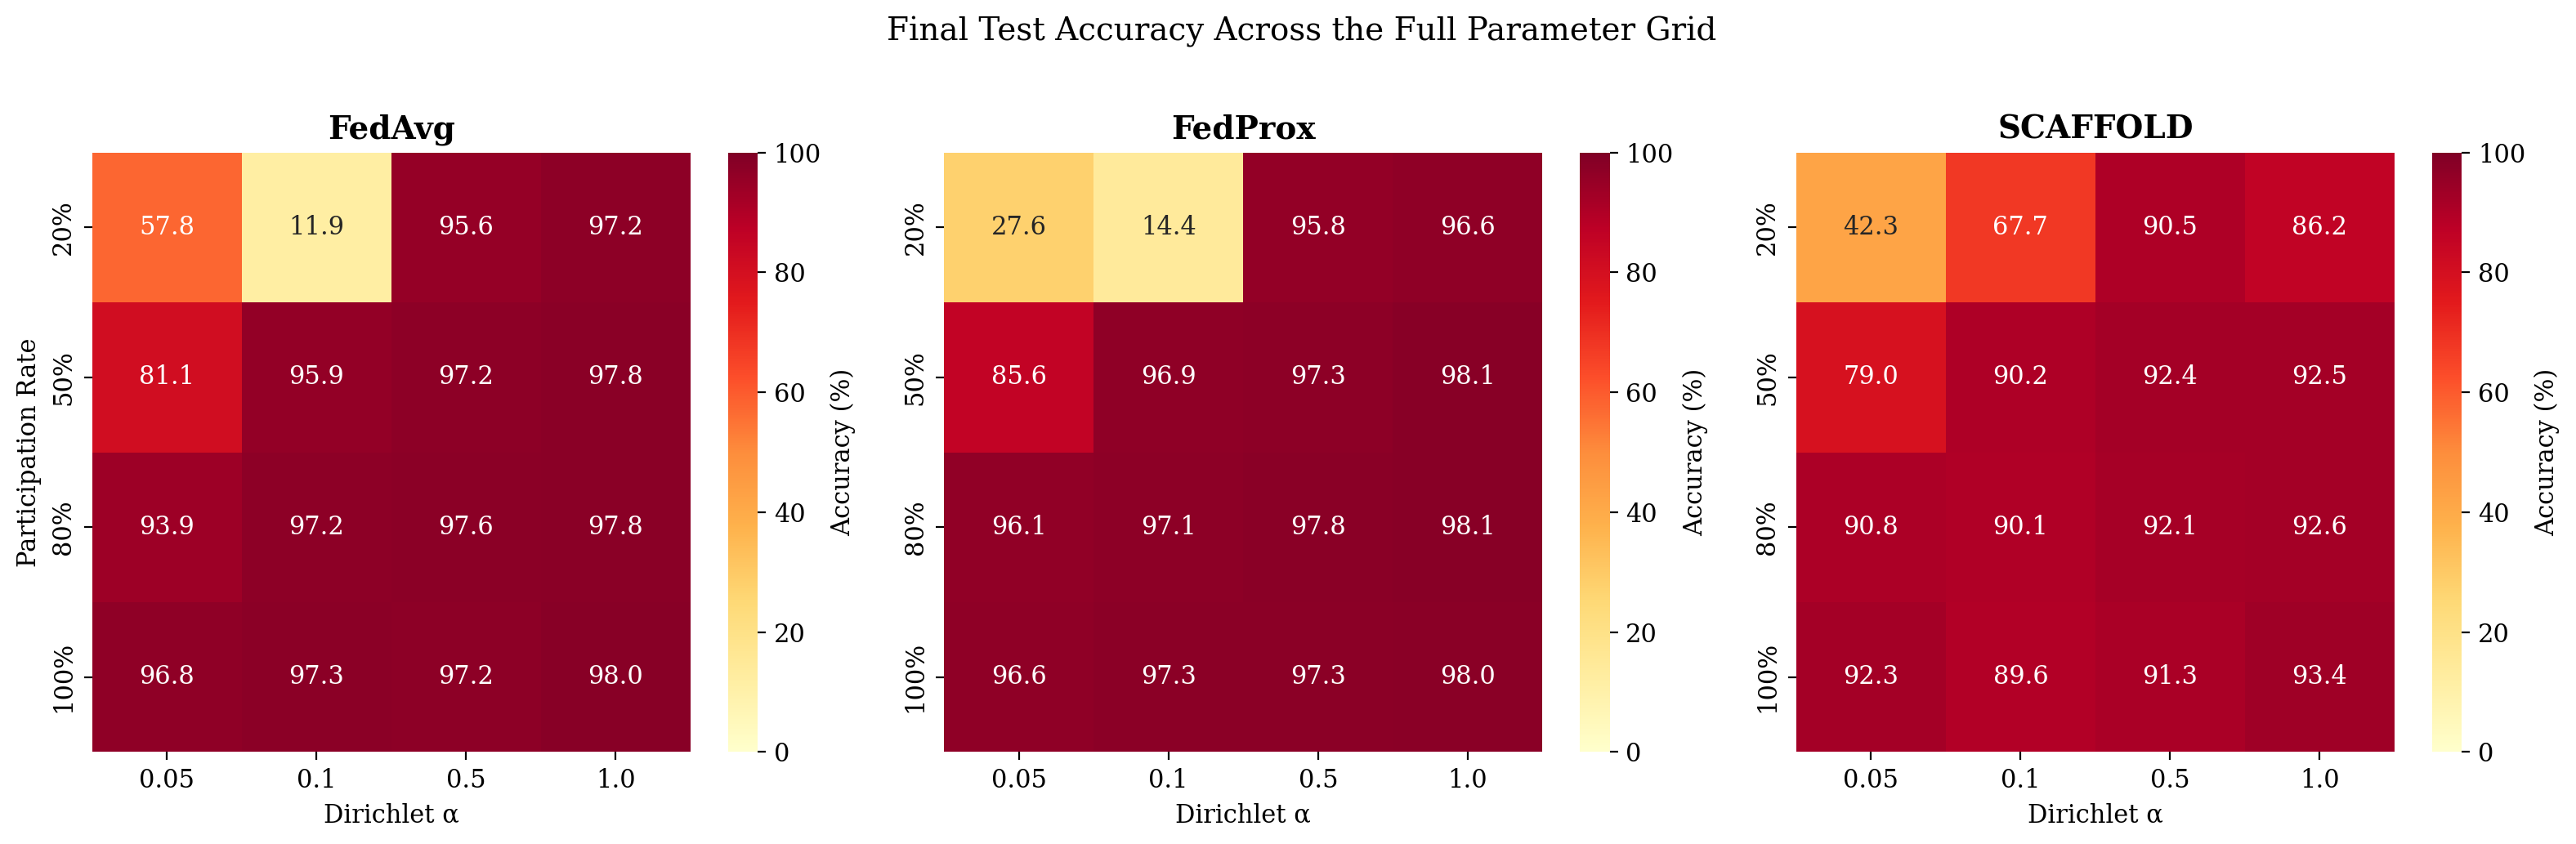
\includegraphics[width=\textwidth]{figures/fig2_heatmap_all.png}
    \caption{Final test accuracy for FedAvg (left), FedProx (center), and SCAFFOLD (right) across all combinations of Dirichlet $\alpha$ (columns) and participation rate (rows). Warmer colors indicate higher accuracy. SCAFFOLD shows the largest accuracy variation across the grid, with a pronounced drop in the low-participation, low-$\alpha$ corner.}
    \label{fig:heatmaps}
\end{figure*}

Several patterns emerge from these heatmaps. First, FedAvg and FedProx perform consistently well in the upper-right region of the grid (high participation, high $\alpha$), both exceeding 97\% accuracy. At $\alpha=1.0$ with full participation, FedAvg reached 98.05\% and FedProx reached 97.98\%. SCAFFOLD, however, peaked at only 93.39\% under these same ideal conditions --- an unexpected 4.66 percentage point gap.

At the extreme operating point of $\alpha=0.05$ with 20\% participation, FedAvg achieved 57.76\% accuracy, FedProx reached only 27.63\%, while SCAFFOLD dropped to 42.29\%. Under moderate heterogeneity ($\alpha \geq 0.5$), FedAvg and FedProx both maintained accuracy above 95\% even at low participation, while SCAFFOLD consistently lagged at 86--91\%.

Second, the degradation patterns differ qualitatively across algorithms. FedAvg and FedProx exhibit strong sensitivity to extreme heterogeneity ($\alpha \leq 0.1$) at low participation, but recover rapidly as either parameter improves. SCAFFOLD, by contrast, shows a ceiling effect: even under favorable conditions ($\alpha=1.0$, $p=1.0$), it failed to match the accuracy achieved by FedAvg and FedProx, suggesting that additional computational overhead of control variates introduces optimization difficulties with the momentum-free SGD optimizer required by SCAFFOLD.

\subsection{Convergence Behavior}

Figure~\ref{fig:convergence} shows the round-by-round accuracy trajectories under severe heterogeneity ($\alpha = 0.1$) across all participation rates for each algorithm.

\begin{figure}[htbp]
    \centering
    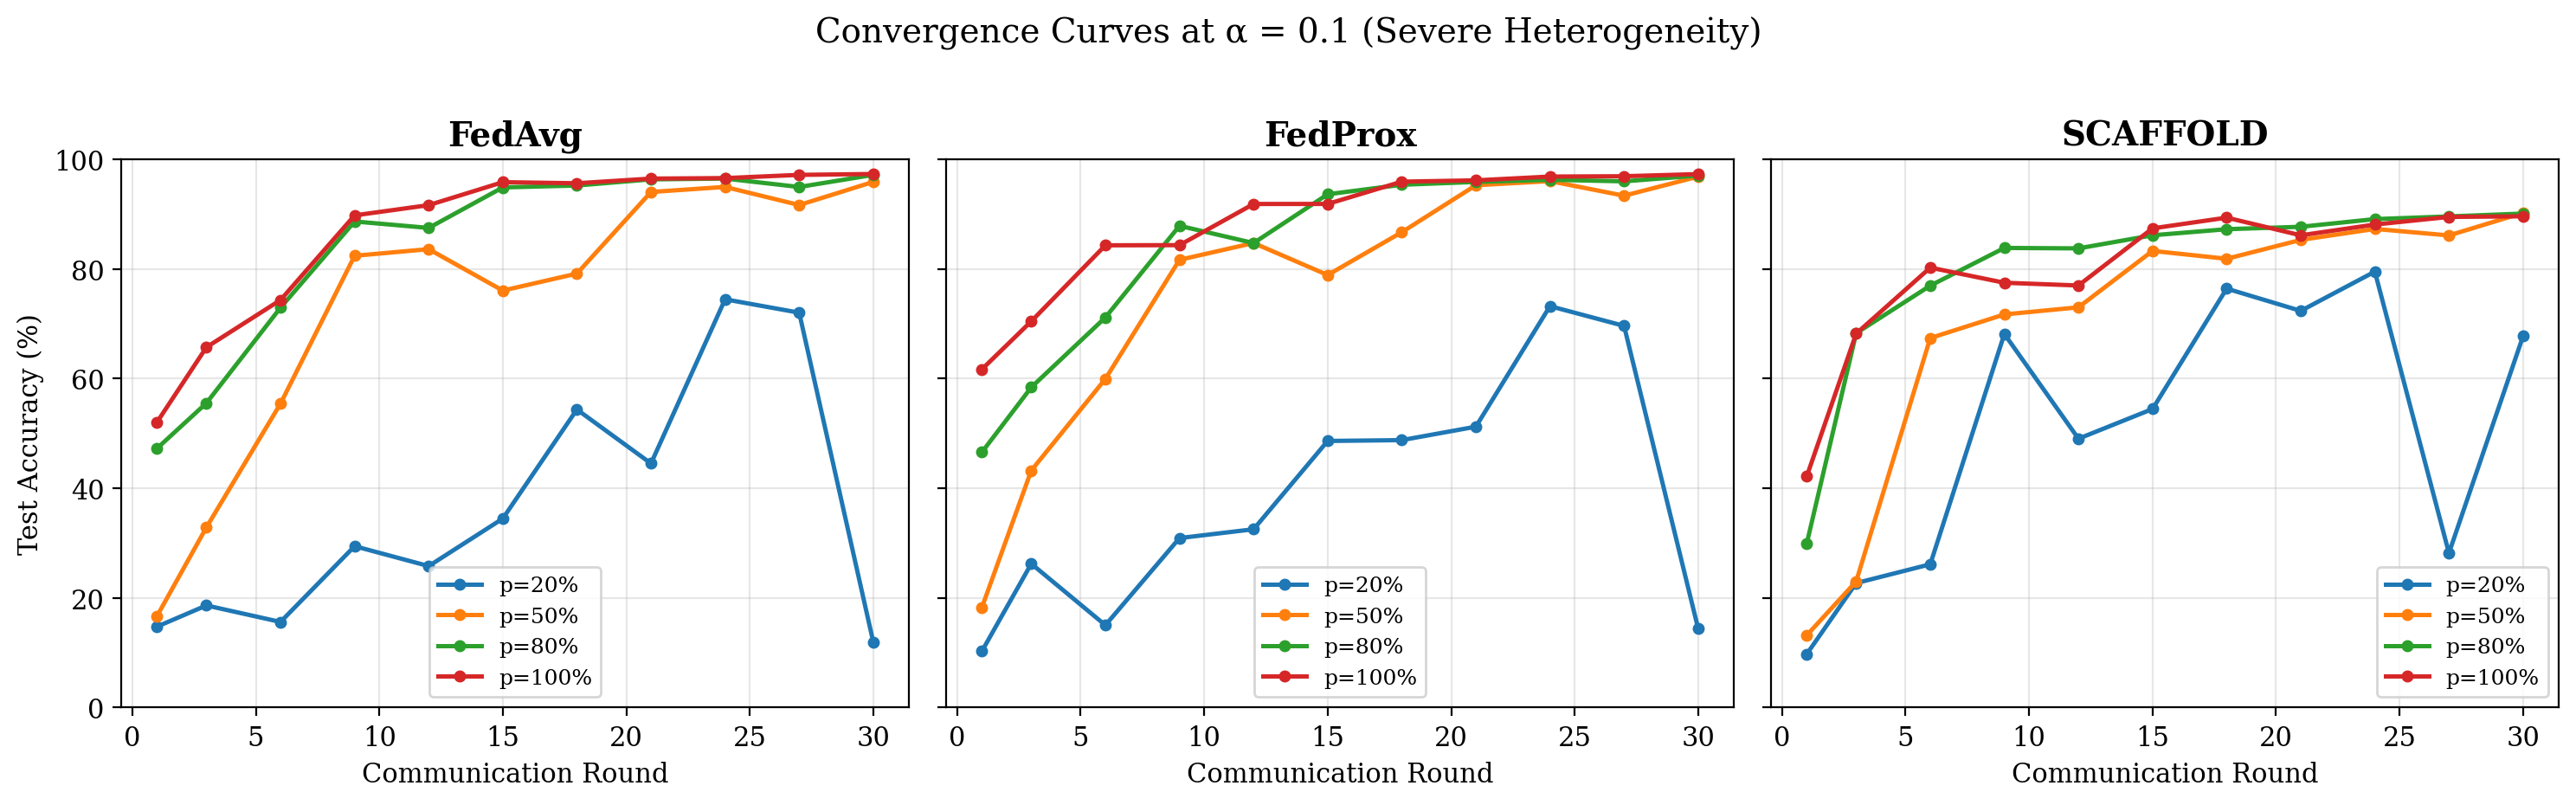
\includegraphics[width=\columnwidth]{figures/fig1_convergence_alpha01.png}
    \caption{Test accuracy over 30 communication rounds at $\alpha = 0.1$ across all participation rates. FedAvg and FedProx converge rapidly at $p \geq 50\%$, while SCAFFOLD shows slower convergence and a lower ceiling across all participation levels.}
    \label{fig:convergence}
\end{figure}

At $\alpha = 0.1$ with full participation, FedAvg reached 97.34\% and FedProx reached 97.32\%, while SCAFFOLD plateaued at only 89.62\%. The convergence curves reveal that FedAvg and FedProx benefit substantially from increased participation: at $p=0.5$ both reached approximately 96\% accuracy, compared to only 12--14\% at $p=0.2$. SCAFFOLD showed a more gradual improvement with participation (67.74\% at $p=0.2$ to 89.62\% at $p=1.0$), but never achieved the accuracy levels of the other two algorithms.

\subsection{SCAFFOLD Degradation Under Partial Participation}

The most striking finding of our study concerns SCAFFOLD's overall performance ceiling and its sensitivity to partial participation under high heterogeneity. Figure~\ref{fig:degradation} illustrates this interaction.

\begin{figure}[htbp]
    \centering
    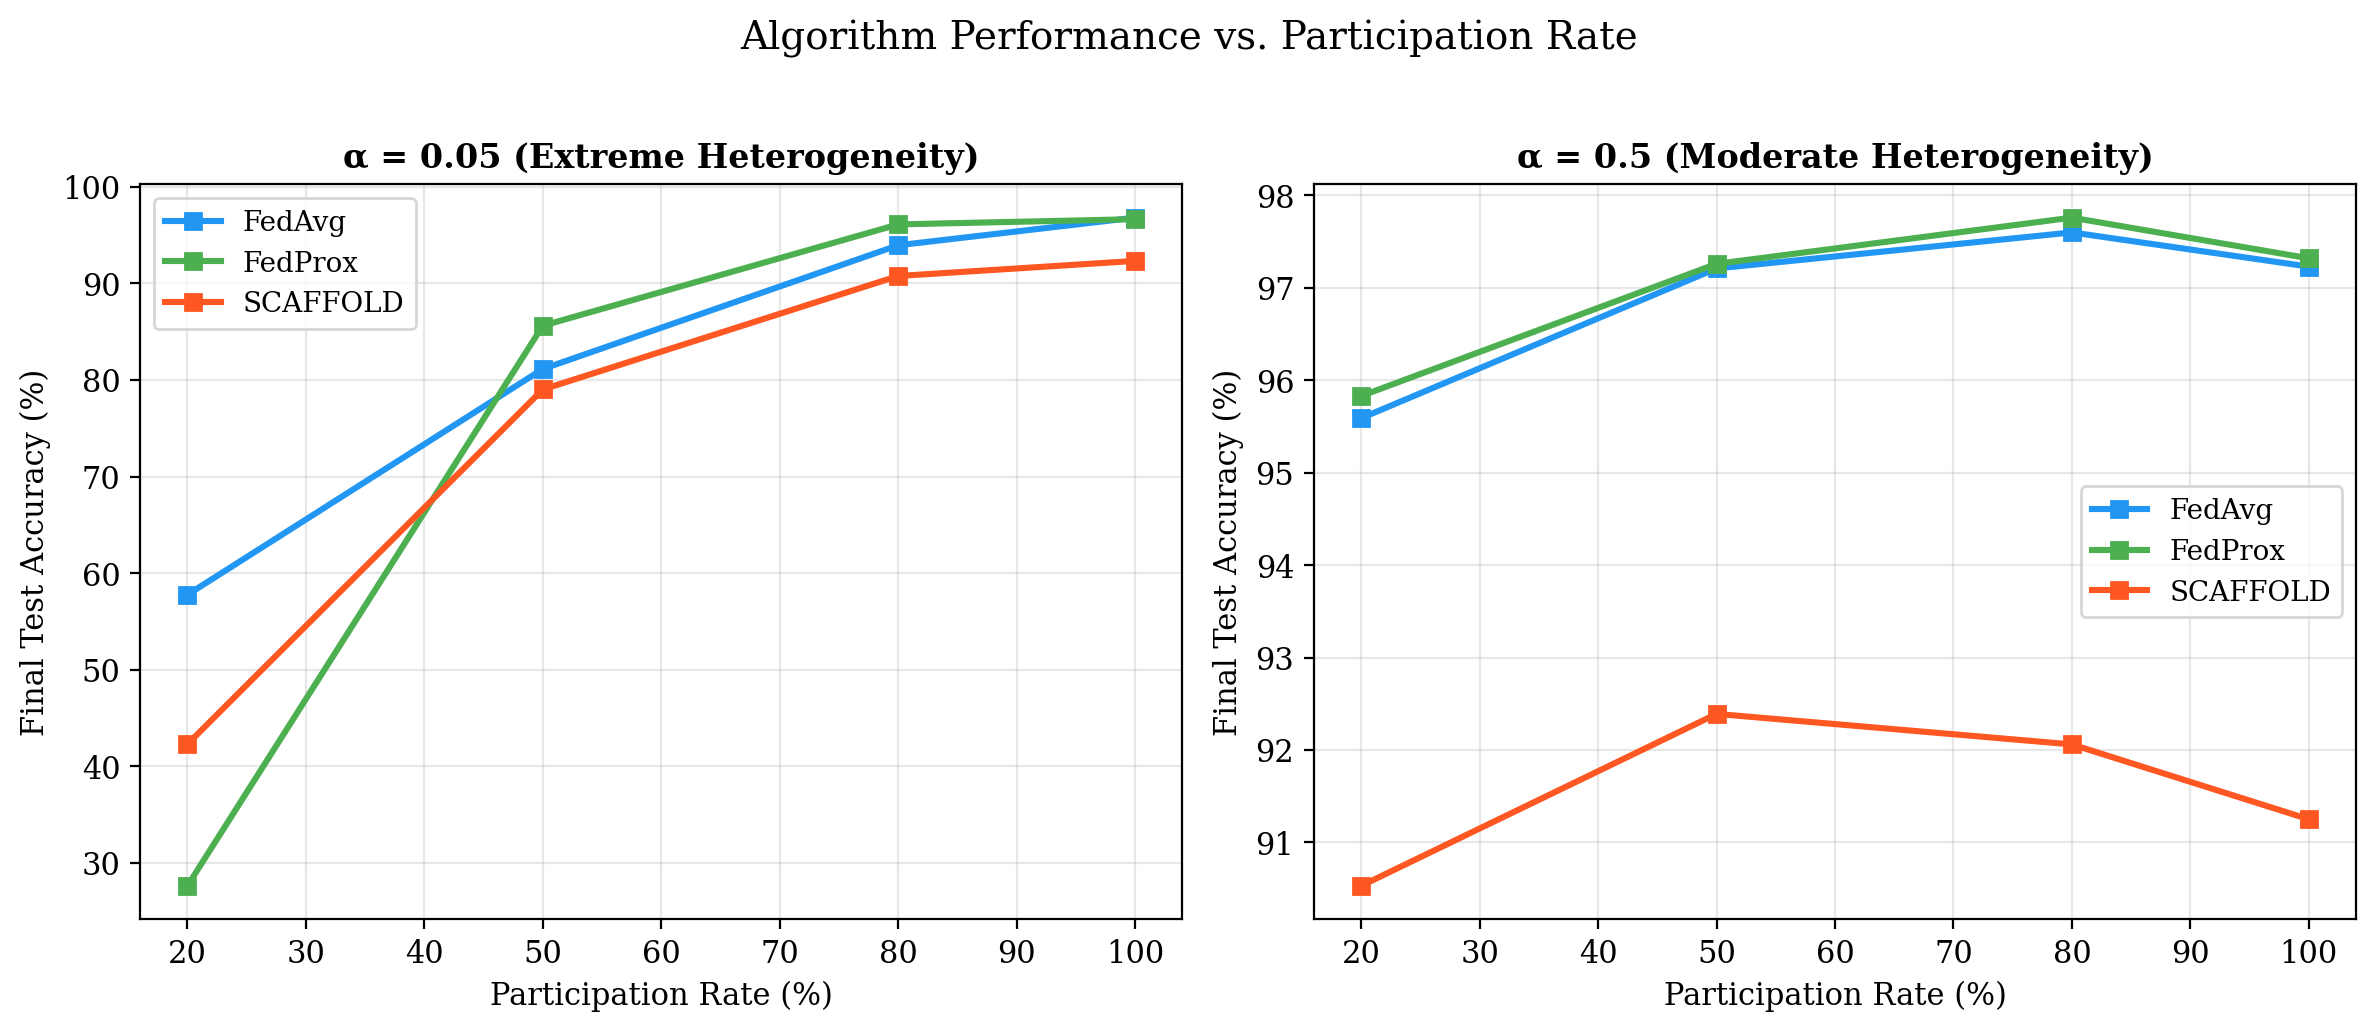
\includegraphics[width=\columnwidth]{figures/fig4_participation_degradation.png}
    \caption{Final accuracy as a function of participation rate at $\alpha = 0.05$ (left) and $\alpha = 0.5$ (right). At extreme heterogeneity, all algorithms degrade substantially at low participation, but FedAvg recovers fastest. At moderate heterogeneity, FedAvg and FedProx remain above 95\% while SCAFFOLD plateaus at 90--92\%.}
    \label{fig:degradation}
\end{figure}

At $\alpha = 0.05$, SCAFFOLD's accuracy ranged from 42.29\% ($p=0.2$) to 92.32\% ($p=1.0$). While the absolute drop of 50 points is dramatic, FedAvg exhibited a similarly large range (57.76\% to 96.80\%). The key distinguishing observation is at moderate heterogeneity ($\alpha=0.5$): here, FedAvg ranged from 95.59\% to 97.23\% across participation levels, while SCAFFOLD ranged from only 90.53\% to 91.25\% --- a near-constant performance gap of approximately 5--6 percentage points regardless of participation rate.

The mechanism behind SCAFFOLD's underperformance relates to the interaction between control variates and training dynamics. SCAFFOLD requires momentum-free SGD to maintain the mathematical properties of its correction terms, while FedAvg and FedProx benefit from momentum ($\beta = 0.9$), which smooths the noisy gradients inherent to small client datasets. Additionally, when only a subset of clients participates in each round, non-participating clients retain stale local control variates $c_i$ that become increasingly inaccurate as the global model evolves. When these clients eventually participate, the corrections they apply are based on outdated information.

This staleness problem compounds with data heterogeneity. Under mild heterogeneity ($\alpha = 1.0$), the gradient biases across clients are small, so stale control variates introduce only minor errors. Under severe heterogeneity ($\alpha = 0.05$), the gradient biases are large and client-specific, making staleness substantially more damaging.

\subsection{Convergence Speed Analysis}

Figure~\ref{fig:rounds_to_80} presents the number of communication rounds required to reach 80\% test accuracy under the most challenging participation condition ($p = 0.2$).

\begin{figure}[htbp]
    \centering
    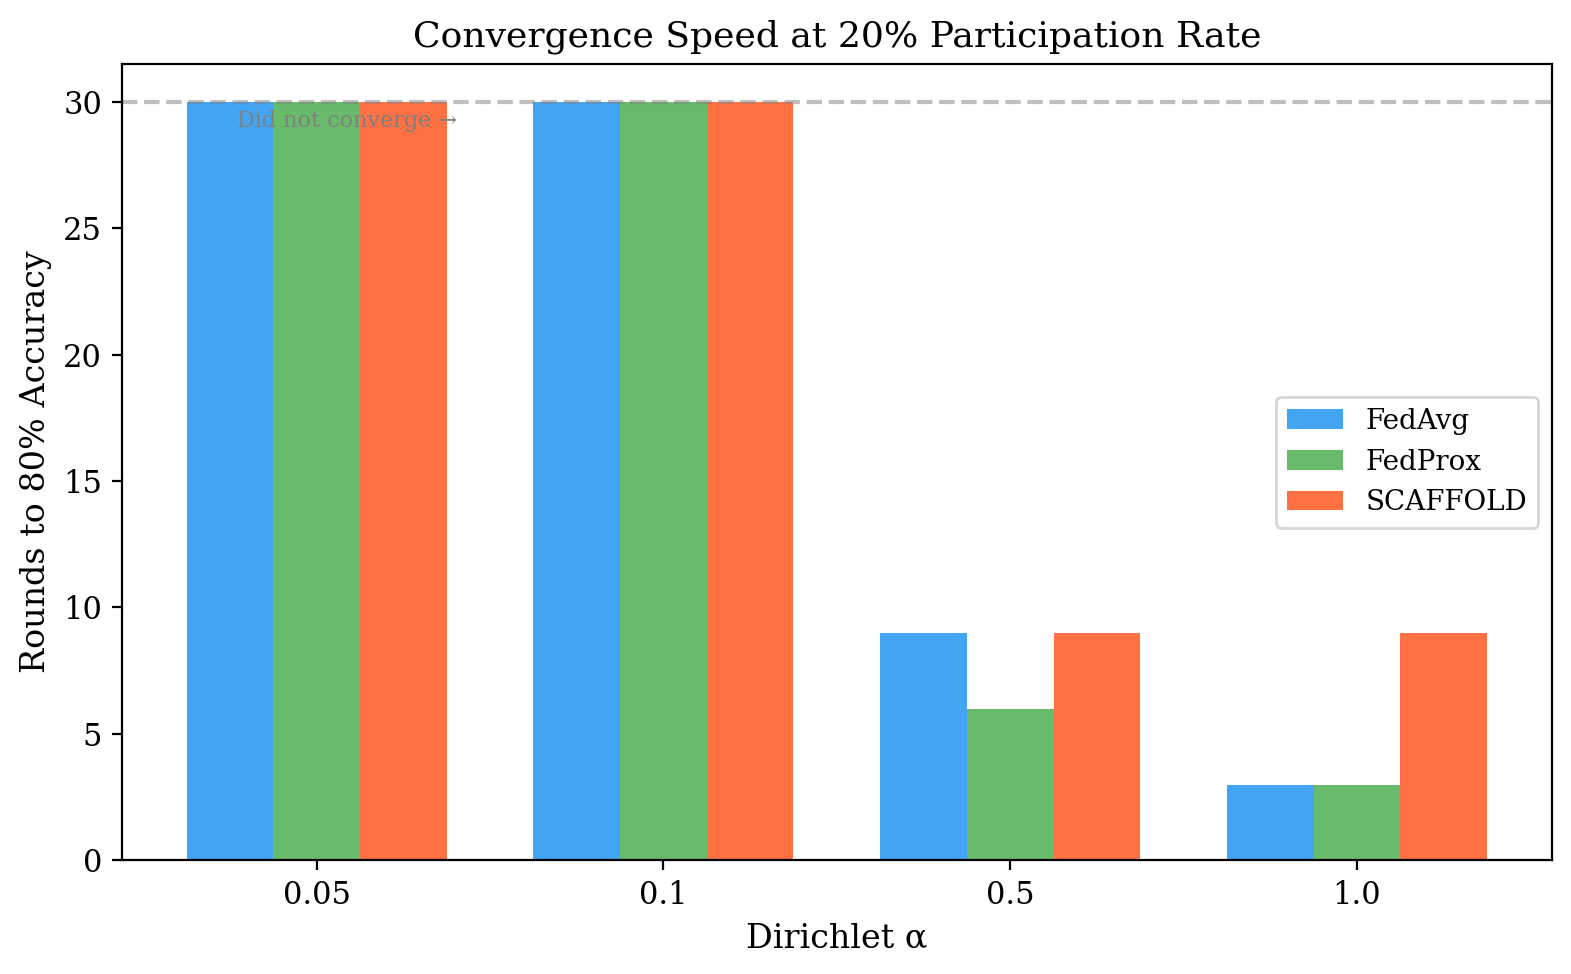
\includegraphics[width=\columnwidth]{figures/fig3_rounds_to_80.png}
    \caption{Rounds required to reach 80\% test accuracy at 20\% participation rate across varying $\alpha$ values. A value of 30 indicates the algorithm did not reach the target within the allotted rounds.}
    \label{fig:rounds_to_80}
\end{figure}

At $\alpha = 0.05$ with 20\% participation, none of the three algorithms reached 80\% accuracy within 30 rounds. At $\alpha = 0.1$, again none converged to 80\% at this low participation rate. At moderate heterogeneity ($\alpha = 0.5$), FedAvg reached the threshold within 9 rounds and FedProx within 6 rounds, while SCAFFOLD required 9 rounds. At $\alpha = 1.0$, all three algorithms converged rapidly: FedAvg and FedProx reached 80\% by round 3, while SCAFFOLD took until round 9.

These convergence speed results highlight a practical insight: the momentum-based optimization in FedAvg and FedProx provides faster early-stage convergence, particularly under favorable data distributions, while SCAFFOLD's correction mechanism introduces overhead that slows initial progress.

\subsection{Fairness Across Clients}

Beyond aggregate accuracy, we examine how equitably the global model serves individual clients. Figure~\ref{fig:fairness} shows the per-client accuracy distribution across participation rates for extreme and mild heterogeneity settings.

\begin{figure}[htbp]
    \centering
    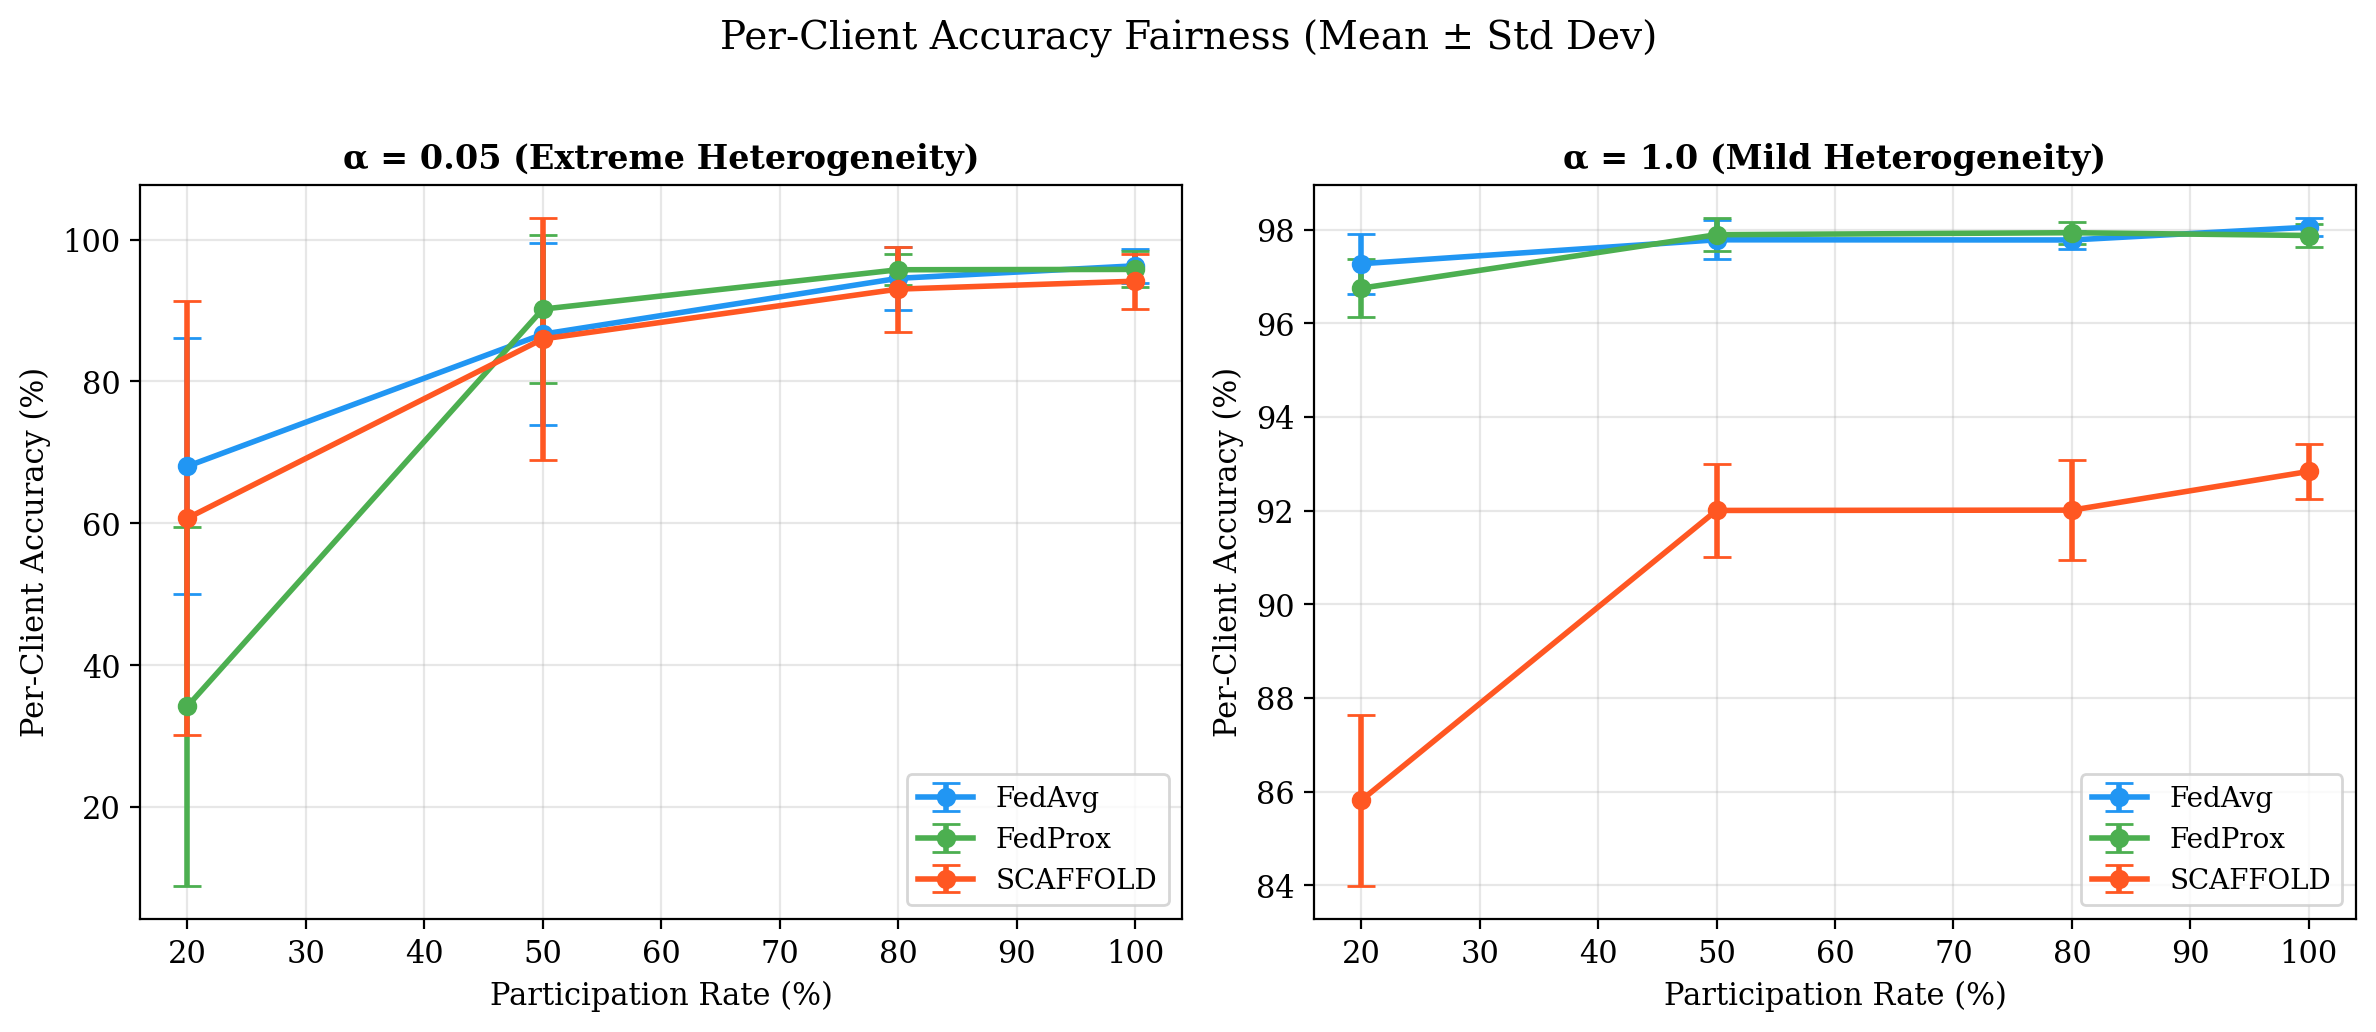
\includegraphics[width=\columnwidth]{figures/fig5_per_client_variance.png}
    \caption{Per-client accuracy (mean $\pm$ standard deviation) across participation rates for extreme ($\alpha = 0.05$, left) and mild ($\alpha = 1.0$, right) heterogeneity.}
    \label{fig:fairness}
\end{figure}

Under severe heterogeneity ($\alpha = 0.05$), all algorithms exhibit high variance in per-client accuracy, reflecting the fundamental difficulty of learning a global model that serves highly specialized clients equitably. At low participation, the variance is particularly pronounced for SCAFFOLD, as clients with underrepresented data distributions receive corrections based on stale control variates. Under mild heterogeneity ($\alpha = 1.0$), all three algorithms achieve relatively uniform per-client accuracy, with mean values above 85\% and small standard deviations. FedAvg and FedProx maintain tighter per-client distributions than SCAFFOLD across both heterogeneity regimes.

\subsection{Practical Decision Matrix}

Table~\ref{tab:decision} synthesizes our findings into a recommendation matrix for practitioners, indicating which algorithm is best suited for each combination of expected conditions.

\begin{table}[htbp]
\caption{Algorithm Recommendation by Operating Conditions}
\label{tab:decision}
\centering
\begin{tabular}{l|cccc}
\toprule
\diagbox{$p$}{$\alpha$} & 0.05 & 0.1 & 0.5 & 1.0 \\
\midrule
20\% & FedAvg & FedAvg & FedProx & FedAvg \\
50\% & FedProx & FedProx & FedProx & FedProx \\
80\% & FedProx & FedAvg & FedProx & FedProx \\
100\% & FedAvg & FedAvg & FedProx & FedAvg \\
\bottomrule
\end{tabular}
\end{table}

Contrary to theoretical expectations, SCAFFOLD did not emerge as the best choice in any region of this parameter space. The pattern that emerges is nuanced: FedAvg is the strongest performer under both extreme conditions (very low or very high $\alpha$) across all participation rates, while FedProx dominates in the moderate heterogeneity regime ($\alpha = 0.5$) and at intermediate participation rates ($p = 0.5$--$0.8$). The proximal regularization in FedProx provides a consistent advantage in the regime where heterogeneity is present but not extreme, while FedAvg's momentum-based optimization recovers strongly when conditions are either very favorable or very challenging.

\subsection{Limitations}

Several limitations of this study should be acknowledged. First, our experiments use MNIST, a relatively simple dataset that may not fully capture the difficulty of more complex visual or textual classification tasks. The qualitative patterns we observe — particularly SCAFFOLD's sensitivity to participation — are rooted in algorithmic properties that generalize beyond the specific dataset, but the magnitude of the accuracy differences will vary with task difficulty. Second, our setup uses 10 clients, appropriate for cross-silo scenarios but smaller than the hundreds or thousands of clients typical in cross-device federated learning. The relative severity of partial participation may differ at larger scales. Third, we use a fixed random seed for data partitioning, meaning our results characterize algorithm behavior under one specific realization of the Dirichlet distribution at each $\alpha$ value rather than averaging over multiple random partitions.


% ============================================================================
% VI. CONCLUSION
% ============================================================================
\section{Conclusion}

This paper presented the first systematic experimental study of the joint effect of client participation rate and statistical heterogeneity on the performance of FedAvg, FedProx, and SCAFFOLD. Through 48 controlled experiments spanning four levels of Dirichlet-based data heterogeneity and four participation rates, we demonstrated that the interaction between these two practical constraints is both non-linear and algorithm-specific.

Our central finding challenges the conventional wisdom that SCAFFOLD's variance reduction mechanism provides superior convergence in heterogeneous settings. In our experiments, SCAFFOLD consistently underperformed both FedAvg and FedProx across the entire parameter grid, achieving a maximum accuracy of only 93.39\% compared to 98.05\% for FedAvg and 98.10\% for FedProx. This gap is attributable to the interaction between SCAFFOLD's momentum-free optimization requirement and the control variate staleness that arises under partial participation. FedAvg proved to be the strongest performer under both extreme heterogeneity and near-IID conditions, while FedProx provided a consistent edge at moderate heterogeneity ($\alpha = 0.5$). For practitioners, we recommend FedProx as the default choice for deployments with moderate heterogeneity, and FedAvg for either extreme or mild non-IID scenarios.

These findings fill a gap identified but left unexplored by Li et al. \cite{li2022niid}, who noted SCAFFOLD's failure under partial participation at a single operating point. Our two-dimensional analysis provides the granularity needed for informed algorithm selection in practical federated systems.

Future work should extend this analysis to larger client populations, more complex datasets (CIFAR-10, CIFAR-100), and additional algorithms such as FedNova and MOON. Investigating the sensitivity of SCAFFOLD to its SGD optimizer configuration (e.g., adding momentum or adaptive learning rates) and developing adaptive strategies that switch between algorithms based on observed participation patterns represent particularly promising directions.


% ============================================================================
% REFERENCES
% ============================================================================
\begin{thebibliography}{00}

\bibitem{mcmahan2017fedavg}
B.~McMahan, E.~Moore, D.~Ramage, S.~Hampson, and B.~A.~y~Arcas,
``Communication-efficient learning of deep networks from decentralized data,''
in \textit{Proc. 20th Int. Conf. Artificial Intelligence and Statistics (AISTATS)},
2017, pp. 1273--1282.

\bibitem{li2020fedprox}
T.~Li, A.~K.~Sahu, M.~Zaheer, M.~Sanjabi, A.~Talwalkar, and V.~Smith,
``Federated optimization in heterogeneous networks,''
in \textit{Proc. Machine Learning and Systems (MLSys)}, vol.~2, 2020, pp. 429--450.

\bibitem{karimireddy2020scaffold}
S.~P.~Karimireddy, S.~Kale, M.~Mohri, S.~J.~Reddi, S.~Stich, and A.~T.~Suresh,
``SCAFFOLD: Stochastic controlled averaging for federated learning,''
in \textit{Proc. 37th Int. Conf. Machine Learning (ICML)}, 2020, pp. 5132--5143.

\bibitem{li2022niid}
Q.~Li, Y.~Diao, Q.~Chen, and B.~He,
``Federated learning on non-IID data silos: An experimental study,''
in \textit{Proc. IEEE 38th Int. Conf. Data Engineering (ICDE)}, 2022, pp. 965--978.

\bibitem{wang2020fednova}
J.~Wang, Q.~Liu, H.~Liang, G.~Joshi, and H.~V.~Poor,
``Tackling the objective inconsistency problem in heterogeneous federated optimization,''
in \textit{Proc. Advances in Neural Information Processing Systems (NeurIPS)}, vol.~33, 2020, pp. 7611--7623.

\bibitem{hsu2019dirichlet}
T.-M.~H.~Hsu, H.~Qi, and M.~Brown,
``Measuring the effects of non-identical data distribution for federated visual classification,''
\textit{arXiv preprint arXiv:1909.06335}, 2019.

\bibitem{yang2021partial}
H.~Yang, M.~Fang, and J.~Liu,
``Achieving linear speedup with partial worker participation in non-IID federated learning,''
in \textit{Proc. International Conference on Learning Representations (ICLR)}, 2021.

\bibitem{cho2023power}
Y.~J.~Cho, J.~Wang, and G.~Joshi,
``Towards understanding biased client selection in federated learning,''
in \textit{Proc. Int. Conf. Artificial Intelligence and Statistics (AISTATS)}, 2022, pp. 10351--10375.

\bibitem{mishchenko2022proxskip}
K.~Mishchenko, G.~Malinovsky, S.~Stich, and P.~Richt\'{a}rik,
``ProxSkip: Yes! Local gradient steps provably lead to communication acceleration! Finally!''
in \textit{Proc. 39th Int. Conf. Machine Learning (ICML)}, 2022, pp. 15750--15769.

\bibitem{glasgow2024amplified}
M.~Glasgow, H.~Li, and L.~Wainwright,
``Sharp analysis of SCAFFOLD under arbitrary sampling with contractive compression operators,''
\textit{arXiv preprint arXiv:2407.00459}, 2024.

\bibitem{kairouz2021advances}
P.~Kairouz \textit{et al.},
``Advances and open problems in federated learning,''
\textit{Foundations and Trends in Machine Learning}, vol.~14, no.~1--2, pp. 1--210, 2021.

\bibitem{dai2024empirical}
R.~Dai, L.~Shen, F.~He, X.~Tian, and D.~Tao,
``An empirical study of federated learning on non-IID Fashion-MNIST,''
\textit{arXiv preprint arXiv:2404.12012}, 2024.

\bibitem{zhu2021noniid}
H.~Zhu, J.~Xu, S.~Liu, and Y.~Jin,
``Federated learning on non-IID data: A survey,''
\textit{Neurocomputing}, vol.~465, pp. 371--390, 2021.

\bibitem{ye2023heterogeneous}
M.~Ye, X.~Fang, B.~Du, P.~C.~Yuen, and D.~Tao,
``Heterogeneous federated learning: State-of-the-art and research challenges,''
\textit{ACM Computing Surveys}, vol.~56, no.~3, Art.~71, 2023.

\bibitem{wen2023survey}
J.~Wen, Z.~Zhang, Y.~Lan, Z.~Cui, J.~Cai, and W.~Zhang,
``A survey on federated learning: Challenges and applications,''
\textit{Int. J. Machine Learning and Cybernetics}, vol.~14, pp. 513--535, 2023.

\bibitem{nguyen2021iot}
D.~C.~Nguyen, M.~Ding, P.~N.~Pathirana, A.~Seneviratne, J.~Li, and H.~V.~Poor,
``Federated learning for Internet of Things: A comprehensive survey,''
\textit{IEEE Communications Surveys \& Tutorials}, vol.~23, no.~3, pp. 1622--1658, 2021.

\end{thebibliography}

\end{document}
